
\section{Wednesday for MAT3006}\index{Wednesday_lecture}
\subsection{Fubini's and Tonell's Theorem}
\paragraph{Motivation}
Given two measurable space 
$(\mathbb{R},\mathcal{M},\diff x)$ and $(\mathbb{R},\mathcal{M},\diff y)$,
we have constructed the product measurable space 
$(\mathbb{R}^2,\mathcal{M}\otimes\mathcal{M},\diff\pi)$.
Suppose $f:\mathbb{R}^2\to[-\infty,\infty]$ is measurable on this space, now we want to show that
\[
\int f(x,y)\diff\pi
=
\int\left(
\int f_y(x)\diff x
\right)\diff y
=
\int
\left(
\int f_x(y)\diff y
\right)
\diff x
\]

\paragraph{Easier Goal}
The proof for the statement above is hard. 
Consider the easier case where $f$ is a simple function first, i.e., 
$f(x,y)=\mathcal{X}_E(x,y), E\in\mathcal{M}\otimes\mathcal{M}$, which follows that
\begin{align*}
\int \mathcal{X}_E(x,y)\diff\pi&=\pi(E)\\
\int(\mathcal{X}_E)_y(x)\diff x
&=
\int \mathcal{X}_{E_y}(x)\diff x
=
m_X(E_y)\\
\int(\mathcal{X}_E)_x(y)\diff y
&=
\int \mathcal{X}_{E_x}(y)\diff x
=
m_Y(E_x)
\end{align*}
Therefore, our easier goal is to show that 
\begin{equation}\label{Eq:13:1}
\pi(E)=\int m_X(E_y)\diff y=\int m_Y(E_x)\diff x,\quad
\forall E\in\mathcal{M}\otimes\mathcal{M}.
\end{equation}


\paragraph{Easiest Goal}
Consider the simplest case where 
$E=A\times B\in\mathcal{M}\otimes\mathcal{M}$, where $A\in\mathcal{M}_X,B\in\mathcal{M}_Y$,
which implies
\begin{itemize}
\item
$\pi(A\times B) = m_X(A)m_Y(B)$
\item
As shown in the figure~(\ref{fig:13:1}), for fixed $y\in Y$,
\[
m_X((A\times B)_y)
=
\left\{
\begin{aligned}
m_X(A),&\quad\text{if $y\in B$}\\
m_X(\emptyset)=0,&\quad\text{if $y\notin B$}
\end{aligned}
\right.
=
m_X(A)\mathcal{X}_B(y)
\]
\begin{figure}[H]
\centering
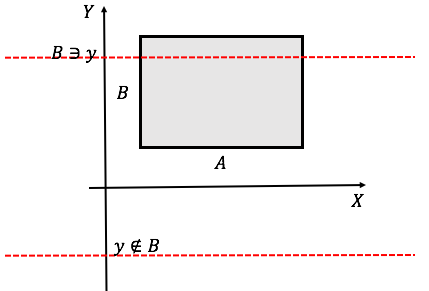
\includegraphics[width=0.5\textwidth]{week13/f_20}
\caption{Illustration for $m_X((A\times B)_y)$}
\label{fig:13:1}
\end{figure}
\end{itemize}
Therefore, we imply
\begin{align*}
\int m_X((A\times B)_y)\diff y  &= \int m_X(A)\mathcal{X}_B(y)\diff y\\
&=
m_X(A)\int \mathcal{X}_B(y)\diff y\\
&=m_X(A)m_Y(B)
\end{align*}
Similarly,
\[
\int m_Y((A\times B)_x)\diff x = m_X(A)m_Y(B).
\]
Therefore, the easiest goal (Eq.~(\ref{Eq:13:1})) holds for $E=A\times B\in \mathcal{M}\times\mathcal{M}$.

\begin{remark}
Generalization from the easier goal to the real goal is trivial, i.e., applying MCT is ok.
The difficulty is that how to show the easier goal (Eq.~(\ref{Eq:13:1})) holds for any $E\in\mathcal{M}\otimes\mathcal{M}$, given that the easier goal (Eq.~(\ref{Eq:13:1})) holds for any $E\in \mathcal{M}\times\mathcal{M}$.
\end{remark}

\begin{definition}[Monotone Class]
Let $X$ be a non-empty set.
A \emph{monotone class} $\mathcal{T}$ is a collection of subsets of $X$ closed under countable increasing unions and countable decreasing intersections, i.e., 
\begin{enumerate}
\item
If $E_i\in\mathcal{T} (i\in\mathbb{N})$ and $E_i\subseteq E_{i+1},\forall i$, then
\[
\bigcup_{i=1}^\infty E_i\in\mathcal{T}
\]
\item
If $F_i\in\mathcal{T} (i\in\mathbb{N})$ with $F_i\supseteq F_{i+1},\forall i$, then
\[
\bigcap_{i=1}^\infty F_i\in\mathcal{T}
\]
\end{enumerate}
\end{definition}
\begin{remark}
Every $\sigma$-algebra is a monotone classs.
In particular, for $X=\mathbb{R}$, the collection of subsets $\mathcal{M}$ and $\mathcal{B}$ are both monotone classes.
\end{remark}


\begin{definition}[Smallest Monotone Class]
For any $S\subseteq\mathcal{P}(X)$, denote
\[
\mathcal{M}(S):=\bigcap_{\text{$\mathcal{T}$ is a monotone class such that $S\subseteq\mathcal{T}$}}\mathcal{T},
\]
which is also the monotone class.
We call $\mathcal{M}(S)$ as the smallest monotone class containing $S$.
\end{definition}
\begin{remark}
It's clear that $\mathcal{M}(S)\subseteq\sigma(S)$, where $\sigma(S)$ is the smallest $\sigma$-algebra containing $S$.

Question: when do we have $\mathcal{M}(S)=\sigma(S)$?
\end{remark}


\begin{theorem}[Monotone Class Theorem]
Let $X$ be a non-empty set.
If $S\subseteq\mathcal{P}(X)$ is an \emph{algebra} (i.e., $E_1,E_2\in S\implies E_1\cup E_2\in S,E_1\cap E_2\in S,E_1^c\in S$), then 
$\mathcal{M}(S)=\sigma(S)$.
\end{theorem}
We skip the proof for the monotone class theorem, but you may refer to the proof in the blackboard.


\begin{example}
\begin{enumerate}
\item
Let $X=\mathbb{R}$, and $S^1=\{\text{all intervals}\}$ is \emph{not} an algebra, e.g.,
\[
[1,2]\in S^1\implies [1,2]^c = (-\infty,1)\cup(2,\infty)\notin S^1.
\]
However, $S=\{\text{finite disjoint union of intervals}\}$ is an algebra.
Therefore, \[\mathcal{M}(S)=\sigma(S):=\mathcal{B} (\text{Borel $\sigma$-algebra}).\]
\item
Let $X=\mathbb{R}^2$, and define
\[
S=
\left\{
\text{finite disjoint union of measurable rectangles }
\bigcup_{i=1}^k(A_i\times B_i)
\middle|~
A_i,B_i\in\mathcal{M}
\right\}
\]
Then $S$ is an algebra, for instance, as shown in the Fig.~(\ref{fig:13:2}), $(A\times B)^c = (A^c\times \mathbb{R})\cup(A\times B^c)$ is a disjoint union of 2 measurable rectangles.
\begin{figure}[H]
\centering
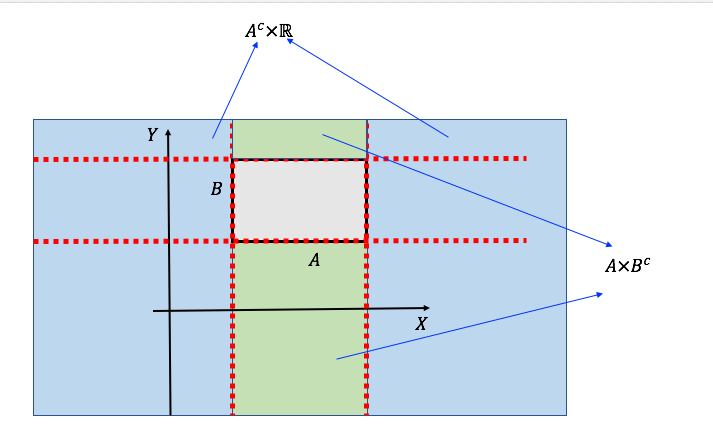
\includegraphics[width=0.5\textwidth]{week13/f_21}
\caption{Illustration for $(A\times B)^c$}
\label{fig:13:2}
\end{figure}

Therefore, $\mathcal{M}(S)=\sigma(S):=\mathcal{M}\otimes\mathcal{M}$
\end{enumerate}
\end{example}

\begin{proposition}
For all $E\in\mathcal{M}\otimes\mathcal{M}$, we have
\begin{equation}\label{Eq:13:2}
\pi(E) = \int m_Y(E_x)\diff x
=
\int m_X(E_y)\diff y\
\end{equation}
\end{proposition}
\begin{proof}
Construct 
\[
\mathcal{A} = \left\{E\in\mathcal{M}\otimes\mathcal{M}
\middle|
\begin{array}{l}
x\mapsto m_Y(E_x)\text{ is a measurable function of $x$}\\
y\mapsto m_X(E_y)\text{ is a measurable function of $y$}\\
\text{Eq.~(\ref{Eq:13:2}) holds}
\end{array}
\right\}
\]
\begin{itemize}
\item
Claim 1: $\mathcal{A}$ is a monotone class
\item
Claim 2: Any finite disjoint union of measurable rectangles is in $\mathcal{A}$:
\[
\bigcup_{i=1}^k(A_i\times B_i)\in\mathcal{A},\quad
k\in\mathbb{N}
\]
\end{itemize}
If claim~(1),(2) holds, then $S\subseteq\mathcal{A}$, where 
\[
S=\{\text{finite disjoint union of measurable rectangles}\}
\]
which follows that 
\[
\mathcal{M}(S)\subseteq\mathcal{A}.
\]
By monotone class theorem, $\sigma(S)=\mathcal{M}(S)\subseteq\mathcal{A}$, i.e.,
\[
\mathcal{M}\otimes\mathcal{M} = \sigma(S)=\mathcal{M}(S)\subseteq\mathcal{A}\subseteq\mathcal{M}\otimes\mathcal{M}
\implies
\mathcal{M}\otimes\mathcal{M}=\mathcal{A}.
\]
Therefore, (\ref{Eq:13:2}) holds for all $E\in\mathcal{A}=\mathcal{M}\otimes\mathcal{M}$.

We left the proof for claim~(1) in next class. Now we give a proof for claim~(2):
\begin{itemize}
\item
For any $E=\cup_{i=1}^k(A_i\times B_i)$, 
\[
m_Y(E_x)=\sum_{i=1}^k m_Y(B_i)\mathcal{X}_{A_i}(x)
\]
is a simple function on $x$, and therefore measurable.
\item
Similarly, 
\[
m_X(E_y) = \sum_{i=1}^km_X(A_i)\mathcal{X}_{B_i}(y)
\]
is also measurable.
\item
By the easiest goal, (\ref{Eq:13:2}) also holds.
\end{itemize}
Therefore, claim~(2) is true.
\end{proof}





















